\begin{figure}[H]
\centering
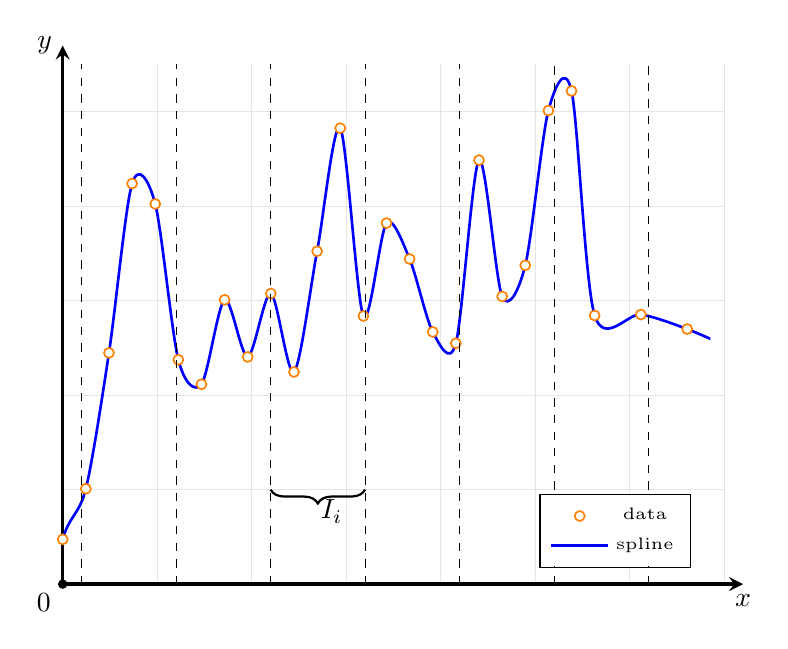
\begin{tikzpicture}[
	scale=1.2,
	axis/.style={
		-stealth,
		very thick
	}
]
% Gitter
\draw[gray!20] (0,0) grid (7,5.5);

% Achsen
\draw[axis] (0,0) -- (0,5.7) node[left]{$\boldsymbol{y}$};
\draw[axis] (0,0) -- (7.2,0) node[below]{$\boldsymbol{x}$};
\fill[black] (0,0) circle[radius=0.05];
\node at(-0.2,-0.2){$\boldsymbol{0}$};

	% Geschweifte Klammer
\draw[
	thick,
	black,
	decorate,
	decoration = {
		brace,
		amplitude = 5pt
	}
] (3.2,1) -- (2.2,1)
	node[
		midway,
		below,
		xshift = 5pt
] {$\boldsymbol{\small I_i}$};


	\begin{axis}[axis lines=none, xmin=67, xmax=95, mark size=1.5pt, legend style={font=\tiny}, legend pos=south east]
	%\pgfplotstableread{data/data.txt}
	%\datatable
	\addplot [mark=*,
			  only marks,
			  mark options={line width=0.5pt, color=orange,fill=white}]
                coordinates{(65,32.54736328)(66,34.39404297)(67,43.53698730)(68,47.45104980)(69,57.97900391)(70,71.09619141)(71,69.52062988)(72,57.44702148)(73,55.55017090)(74,62.09375000)(75,57.66784668)(76,62.57556152)(77,56.50366211)(78,65.85742188)(79,75.39172363)(80,60.83923340)(81,68.03527832)(82,65.25524902)(83,59.60485840)(84,58.72167969)(85,72.91284180)(86,62.35473633)(87,64.76342773)(88,76.75659180)(89,78.27209473)(90,60.87939453)(92,60.94970703)(94,59.82568359)(96,58.27001953)
                };
                \addlegendentry{data}
    
    \addplot [smooth,
			  color=blue,
			  thick]
                coordinates{(65,32.54736328)(66,34.39404297)(67,43.53698730)(68,47.45104980)(69,57.97900391)(70,71.09619141)(71,69.52062988)(72,57.44702148)(73,55.55017090)(74,62.09375000)(75,57.66784668)(76,62.57556152)(77,56.50366211)(78,65.85742188)(79,75.39172363)(80,60.83923340)(81,68.03527832)(82,65.25524902)(83,59.60485840)(84,58.72167969)(85,72.91284180)(86,62.35473633)(87,64.76342773)(88,76.75659180)(89,78.27209473)(90,60.87939453)(92,60.94970703)(94,59.82568359)(96,58.27001953)
                };
                \addlegendentry{spline}
	\end{axis}
	\draw[dashed] (0.2,0) -- (0.2,5.5);  
	\draw[dashed] (1.2,0) -- (1.2,5.5); 
	\draw[dashed] (2.2,0) -- (2.2,5.5);  
	\draw[dashed] (3.2,0) -- (3.2,5.5); 
	\draw[dashed] (4.2,0) -- (4.2,5.5); 
	\draw[dashed] (5.2,0) -- (5.2,0.19);  
	\draw[dashed] (6.2,0) -- (6.2,0.19);  
	\draw[dashed] (5.2,1) -- (5.2,5.5);  
	\draw[dashed] (6.2,1) -- (6.2,5.5);  
	
	%\draw[<-,->] (2.2,1) -- (3.2,1) node[below, midway] {\small $I_i$};
	


\end{tikzpicture}
\caption[Anwendung der \textit{Spline}-Regression]{Anwendung der \textit{Spline}-Regression\protect\footnotemark}
\label{splineZoom}
\end{figure}
\footnotetext{Eigene Darstellung: Vergrößerung der Punktewolke aus \vref{pr} im Wertebereich $x_1$ bis $x_2$.}